\subsection{Απόδοση Γραφικών σε Έμμεσες Διαφορίσιμες Επιφάνειες}
\label{section:neuralImplicitRendering}
Παρακάτω δίνεται μια συνεκτική περιγραφή του αλγορίθμου αποτύπωσης εκπαιδεύσιμης αναπαράστασης.
Ένας αλγόριθμος αποτύπωσης \cite{sitzmann2020scene}, μιας δεδομένης αναπαραστώμενης \enit{3D} σκηνής $\Phi$. Ο Αλγόριθμος που συμβολίζεται με $\Theta$, ο οποίος αντιστοιχίζει μια αναπαράσταση σκηνής $\Phi$ καθώς και τις εξωτερικές $\mathbf{K}$ και εσωτερικές $\mathbf{E}$ παραμέτρους της κάμερας (βλ. για το σύστημα κάμερας στο Κεφ.\ref{chapter:appendix}) σε μια εικόνα $\mathcal{I}$ περιγράφεται ως εξής:
$$
\Theta: \mathcal{X} \times \mathbb{R}^{3 \times 4} \times \mathbb{R}^{3 \times 3} \rightarrow \mathbb{R}^{H \times W \times 3}, \quad(\Phi, \mathbf{E}, \mathbf{K}) \mapsto \Theta(\Phi, \mathbf{E}, \mathbf{K})=\mathcal{I},
$$
όπου $\mathcal{X}$ είναι ο χώρος όλων των συναρτήσεων $\Phi$.
Η βασική επιπλοκή στην απόδοση μιας σκηνής $\Phi$, είναι ότι η γεωμετρία αναπαρίσταται έμμεσα. Η επιφάνεια ενός ξύλινου τραπεζιού, για παράδειγμα, ορίζεται από τον υποχώρο του $\mathbb{R}^3$ όπου το $\Phi$ υφίσταται μια αλλαγή από ένα διάνυσμα χαρακτηριστικών που αναπαριστά τον ελεύθερο χώρο σε ένα που αναπαριστά το ξύλο. Αυτό σκοπεύει και να βελτιώσει και η παρούσα εργασία.

Για να αποτυπώσουμε ένα μεμονωμένο εικονοστοιχείο στην εικόνα που παρατηρείται από μια εικονική κάμερα, πρέπει να λύσουμε επομένως δύο υπό προβλήματα: (i) την εύρεση των παγκόσμιων συντεταγμένων των τομών των αντίστοιχων ακτίνων της κάμερας με τη γεωμετρία της σκηνής και (ii) την αντιστοίχηση του διανύσματος χαρακτηριστικών $\mathbf{v}$ σε αυτή τη χωρική συντεταγμένη σε ένα χρώμα και την προβολή στην εικόνα.

\subsubsection{Αλγόριθμος ανίχνευσης των Τομών Ακτίνων}
Για το κομμάτι εύρεσης των τομών των ακτίνων έγινε παραπάνω μια νύξη στον αλγόριθμο \enit{Sphere Tracing} δεδομένης γεωμετρίας της σκηνής. Θα μπορούσε να προταθεί ένα πιο εξελιγμένο νευρωνικό δίκτυο που θα εφάρμοζε ένα νευρωνικό αλγόριθμο βάδισης ακτίνων με εκπαιδεύσιμο, προσαρμοστικό μέγεθος βήματος για την εύρεση των τομών των ακτίνων με τη γεωμετρία της σκηνής. Περισσότερα στο Παράρτημα Α [Κεφάλαιο \ref{chapter:appendix}].

\subsubsection{Δίκτυο Χρωματισμού Εικονοστοιχείων}
\subsubsection{Δίκτυο που κάνει χρήση BRDF \cite{matusik2003data}}
Το δίκτυο που αφορά τον χρωματισμό εικονοστοιχείων, αποτελεί αντιστοίχηση του διανύσματος χαρακτηριστικών σε αυτή την χωρική συντεταγμένη σε ένα χρώμα και βασικό στέλεχος του δικτύου απόδοσης \enit{Rendering Network}. Αυτό το δίκτυο στην κλασσική περίπτωση μπορεί να υλοποιεί μια συνάρτηση κατανομής της αμφίδρομης ανάκλασης \enit{BRDF}(\enit{Bidirectional Reflectance Distribution Function}).

\begin{figure}[ht]
    \centering
    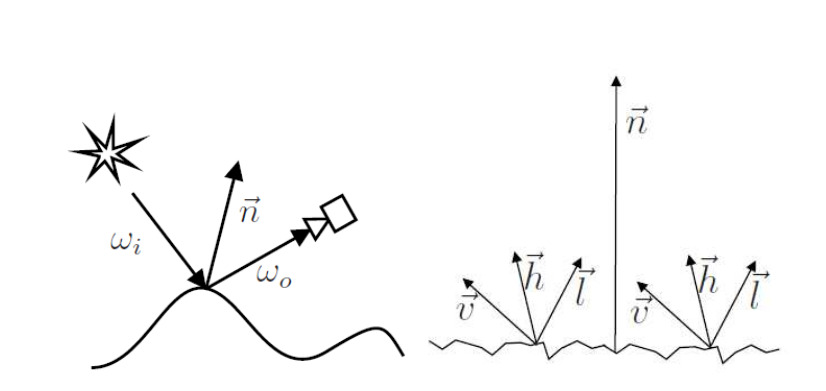
\includegraphics[width=.4\linewidth]{images/chapter2_img/BRDF_Diagram.jpg}
    \caption{Διάγραμμα που δείχνει τα διανύσματα που ορίζουν την BRDF Πηγή \cite{6109209}}
    \label{fig:BRDF}
\end{figure}
Η συνάρτηση BRDF  $\mathcal{B}(\hat{x},\hat{n},\omega^i,\omega^o)$ περιγράφει το μέρος της ανακλώμενης ακτινοβολίας (δηλαδή της ηλεκτρομαγνητικής ροής του φωτός) σε κάποιο μήκος κύματος (δηλαδή το χρώμα) η οποία φεύγει από το σημείο $\chi$  με κανονικό διάνυσμα $\vec{n}$  κατά κατεύθυνση $\omega^o$  σε σχέση με την προσπίπτουσα ακτινοβολία από την κατεύθυνση $\omega^i$ . Η BRDF  επίσης βασίζεται επίσης στο κανονικό διάνυσμα $\vec{n}$ στο σημείο της επιφάνειας (βλ.\ref{chapter:appendix}). Οι πηγές φωτός περιγράφονται από την συνάρτηση $L^e\left(\hat{\boldsymbol{x}},\boldsymbol{\omega}^o\right)$  και δίνουν το μέτρο της ακτινοβολίας που πηγάζει από την φωτεινή πηγή σε κάποιο μήκος κύματος στο σημείο $x$ κατά την κατεύθυνση του $\omega^{o}$ 
Η ολοκλήρωση της BRDF σε καθορισμένες στερεές γωνίες πρόσπτωσης και ανάκλασης ορίζει την ανακλαστικότητα, η οποία μπορεί εύκολα να συσχετιστεί με την απορροφητικότητα (ή την ικανότητα εκπομπής) ενός υλικού. Συνεπώς η συνολική εξίσωση αποτύπωσης δίνεται από τον εξής τύπο: 
\begin{equation}
    L\left(\hat{\boldsymbol{x}},\boldsymbol{\omega}^o\right)=L^e\left(\hat{\boldsymbol{x}},\boldsymbol{\omega}^o\right)+\int_0 B\left(\hat{\boldsymbol{x}}, \hat{\boldsymbol{n}},\boldsymbol{\omega}^i,\boldsymbol{\omega}^o\right) L^i\left(\hat{\boldsymbol{x}},\boldsymbol{\omega}^i\right)\left(\hat{\boldsymbol{n}} \cdot\boldsymbol{\omega}^i\right) d\boldsymbol{\omega}^i=M_0(\hat{\boldsymbol{x}}, \hat{\boldsymbol{n}}, \boldsymbol{v})
    \label{eq:rendering}
\end{equation}

Αυτό είναι και το μοντέλο που χρησιμοποιεί και το  [IDR \cite{yariv2020multiview}] το οποίο υιοθετείται για την απόδοση σκηνής.
\subsubsection{Χρήση Ογκομετρικού Μοντέλου Ακτινοβολίας \enit{NeRF} \cite{mildenhall2020nerf}}
Πολλά μοντέλα διαχειρίζονται το πρόβλημα της ακτινοβολίας χρησιμοποιώντας ως είσοδο \enit{5D} (πέντε διαστάσεων). Αυτά τα μοντέλα υπολογίζουν την εκ λαμβανόμενη ακτινοβολία  για κάθε ακτίνα που περνά από τον καμβά της εικόνας σε όλο το μήκος της μέσω της κλασσικής εξίσωσης ογκομετρικής απόδοσης\ref{eq:volumetricRenderingEquation}.
\begin{definition} Νeural Volume Rendering
    Η νευρωνική απόδοση όγκου αναφέρεται σε μεθόδους που παράγουν εικόνες με την ιχνηλάτηση μιας ακτίνας στη σκηνή και την ολοκλήρωση κατά το μήκος της ακτίνας. Συνήθως ένα νευρωνικό δίκτυο όπως ένα πολυεπίπεδο perceptron κωδικοποιεί μια συνάρτηση από τις τρισδιάστατες συντεταγμένες της ακτίνας σε ποσότητες όπως η πυκνότητα και το χρώμα, οι οποίες ενσωματώνονται για να προκύψει μια εικόνα. Χρησιμοποιείται κατ' εξοχήν στα μοντέλα NeRF
\end{definition}
Πρακτικά σύμφωνα με το NeRF \cite{mildenhall2020nerf}, δεδομένης συνάρτησης πυκνότητας όγκου , το αναμενόμενο χρώμα που γυρνά στην κάμερα $C(\textbf{r})$ κατά την διεύθυνση της ακτίνας $\textbf{r}(t) = \textbf{o} + t\textbf{d}$ με κοντινά και μακριά όρια $t_n,t_f$ δίνεται από την παρακάτω ολοκλήρωση:
\begin{equation}
    C(\mathbf{r})=\int_{t_n}^{t_f} T(t) \sigma(\mathbf{r}(t)) \mathbf{c}(\mathbf{r}(t), \mathbf{d}) d t,
    \label{eq:volumetricRenderingEquation}
\end{equation}
 
$\text { οπού } T(t)=\exp \left(-\int_{t_n}^t \sigma(\mathbf{r}(s)) d s\right)$ αναφέρεται στην συνολική διαφάνεια ή διαπερατότητα φωτός κατά μήκος της ακτίνας\footnote{αυτό είναι έμμεσο πεδίο διαφάνειας που υπολογίζεται σε μοντέλα ογκομετρικής απόδοσης}.

Το σημαντικό με τα ογκομετρικά μοντέλα είναι πως δεν χρειάζονται απαραίτητα επίβλεψη μάσκας για την θέση του αντικειμένου στην σκηνή.  Μπορούν να ξεκινήσουν από ακατέργαστα σημεία του τρισδιάστατου χώρου, με τυχαία αρχικοποίηση παραμέτρων κάμερας και να εκτιμήσουν το πεδίο ακτινοβολίας στην πορεία της ακτίνας, χωρίς να αποκλίνουν.

Η παρούσα εργασία ασχολείται πάνω στο κομμάτι της διαφορίσιμης αποτύπωσης που δεν αφορά όμως τέτοιου είδους δίκτυα. Χρειάζεται ο έλεγχος στο επίπεδο της φωτογραφίας με χρήση δυαδικής μάσκας (\enit{object masked rendering}) για καλύτερη σύγκλιση. Παράλληλα, οι εξωτερικές παράμετροι της κάμερας (\ref{appendix:camerasystem}), πρέπει να μη έχουν αρχικοποιηθεί με τυχαίο τρόπο αλλά μπορούν εκπαιδευτούν μαζί με το δίκτυο. Μια αναλυτική περιγραφή της μεθόδου που ακολουθείται περιγράφεται στην μεθοδολογία(Κεφ. \ref{chapter:implementations}).
\clearpage